\documentclass[11pt,a4paper]{article}
\usepackage[a4paper,left=24mm,right=14mm,top=15mm,bottom=15mm]{geometry}
\usepackage{fontspec}
\setmainfont{Comic Neue}
\usepackage{amsmath,amssymb}
\usepackage{xcolor}
\usepackage{tikz}
\usepackage{eso-pic}
\usepackage{enumitem}
\usepackage[most]{tcolorbox}
\usepackage{fancyhdr}
\usepackage{titlesec}
\usepackage{array}
\usepackage{microtype}
\definecolor{Ink}{HTML}{D62B25}
\definecolor{InkDark}{HTML}{B51F1A}
\definecolor{Grid}{HTML}{D8DCDD}
\definecolor{Paper}{HTML}{FFFCF7}
\definecolor{Hole}{HTML}{9B5B28}
\color{Ink}
\setlength{\parindent}{0pt}
\setlength{\parskip}{4pt}
\linespread{1.08}
\setlist[itemize]{leftmargin=7mm,itemsep=2pt,topsep=2pt,label=\textcolor{Ink}{$\bullet$}}
\pagestyle{fancy}
\fancyhf{}
\fancyfoot[C]{\textcolor{Ink}{\thepage}}
\renewcommand{\headrulewidth}{0pt}
\renewcommand{\footrulewidth}{0pt}
\newcommand{\sourceTag}[1]{\hfill\textcolor{InkDark}{\footnotesize Feuille source #1/21}}
\newcommand{\Title}[1]{\begin{center}\vspace*{-2mm}{\fontsize{19}{22}\selectfont\bfseries\itshape #1}\end{center}\vspace{-2mm}\noindent\rule{\linewidth}{0.7pt}\vspace{3mm}}
\newcommand{\Sub}[1]{\vspace{2mm}{\fontsize{13.5}{15}\selectfont\bfseries\itshape #1}\par\vspace{1mm}\noindent\rule{0.58\linewidth}{0.45pt}\vspace{1mm}}
\newtcolorbox{formule}{colback=Paper,colframe=Ink,boxrule=0.7pt,arc=0mm,left=3mm,right=3mm,top=1.5mm,bottom=1.5mm,center}
\newcommand{\Note}[1]{\begin{tcolorbox}[colback=Paper,colframe=InkDark,boxrule=0.45pt,arc=0mm,left=3mm,right=3mm,top=1mm,bottom=1mm]\small #1\end{tcolorbox}}
\newcommand{\newnote}{\clearpage}
\AddToShipoutPictureBG{%
\begin{tikzpicture}[remember picture,overlay]
  \fill[Paper] (current page.south west) rectangle (current page.north east);
  \draw[Grid,line width=0.16pt,step=5mm] (current page.south west) grid (current page.north east);
  \draw[Ink!35,line width=0.35pt] ([xshift=17mm]current page.south west) -- ([xshift=17mm]current page.north west);
  \foreach \yy in {0.18,0.50,0.82} {\fill[Hole] ([xshift=5.5mm,yshift=\yy\paperheight]current page.south west) circle (1.9mm);}
\end{tikzpicture}%
}
\begin{document}

% Cover
\thispagestyle{empty}
\vspace*{24mm}
\begin{center}
{\fontsize{27}{31}\selectfont\bfseries\itshape Des extrema classiques\\[3mm]au calcul des variations}\par
\vspace{5mm}\rule{150mm}{0.9pt}\vspace{7mm}
{\fontsize{17}{20}\selectfont\itshape Réécriture fidèle, corrigée et réorganisée\\des 21 feuilles manuscrites fournies}\par
\vspace{12mm}
\begin{formule}
\centering\Large De la pente et des extrema à l'équation d'Euler--Lagrange
\end{formule}
\vspace{12mm}
{\large Fermat -- Descartes -- Newton -- Leibniz -- Bernoulli -- Euler}
\end{center}
\vfill
\Note{Principe de cette version : aucune feuille n'est supprimée ni absorbée dans un résumé global. Chaque feuille source reçoit sa propre page de réécriture. Les fautes de français et les erreurs de notation sont corrigées, mais le fil d'idées et les calculs présents dans les notes sont conservés.}
\vspace{10mm}

% Plan
\newnote
\Title{Plan et ordre de réécriture}
Cette version remet les 21 feuilles dans un ordre pédagogique continu. Le numéro de la feuille source reste indiqué en haut de chaque page pour vérifier qu'aucune n'a disparu.
\begin{enumerate}[leftmargin=8mm,itemsep=2.6pt]
\item Base logique : réels, petites variations, proportionnalité. \textit{(source 1)}
\item Courbe, pente et point stationnaire. \textit{(sources 12, 13)}
\item Tangentes et question des extrema : vers Fermat. \textit{(sources 2, 3)}
\item Descartes et géométrie analytique. \textit{(source 4)}
\item Sommet d'une parabole par symétrie algébrique. \textit{(source 6)}
\item Newton : fluxions et mouvement. \textit{(sources 14, 15, 5)}
\item Leibniz : différentiels et dérivée. \textit{(sources 17, 16)}
\item Approximation locale : $f(x+dx)\approx f(x)+f'(x)dx$. \textit{(source 10)}
\item Bernoulli et la brachistochrone. \textit{(sources 19, 18)}
\item Euler : faire bouger une courbe. \textit{(sources 7, 8, 9)}
\item Première variation, intégration par parties et Euler--Lagrange. \textit{(sources 21, 20)}
\item Retour au problème physique et principe de minimisation. \textit{(source 11)}
\end{enumerate}
\Note{L'ordre pédagogique est amélioré, mais le contenu de chaque source est gardé sur une page dédiée.}

% Source 1
\newnote\sourceTag{1}\Title{Base logique : continuité des réels et proportionnalité}
\Sub{1. Les nombres réels comme espace de comparaison}
Sur l'ensemble des nombres réels $\mathbb{R}$, on peut comparer les grandeurs grâce à l'ordre : pour deux nombres, l'un est plus petit, égal ou plus grand que l'autre. Cela permet de parler de minimum, de maximum et d'écart entre deux valeurs.
\begin{itemize}
\item Une petite différence s'écrit par exemple : $(x+dx)-x=dx$.
\item On peut considérer des valeurs arbitrairement proches l'une de l'autre.
\item La stabilité de $\mathbb{R}$ pour l'addition et la multiplication permet de multiplier un petit déplacement $dx$ par un nombre réel.
\end{itemize}
\Sub{2. Changement local proportionnel}
L'idée de la feuille est la suivante : lorsqu'un changement $dx$ est très petit, le changement local principal d'une quantité $y$ peut être représenté, au premier ordre, comme un nombre réel multiplié par $dx$.
\begin{formule}
\[\Delta y \approx k\,dx\]
\end{formule}
Dans le calcul différentiel moderne, ce coefficient local deviendra la dérivée $f'(x)$ lorsque $y=f(x)$.
\Sub{3. Deux grandeurs proportionnelles}
Deux grandeurs $A$ et $B$ sont proportionnelles s'il existe une constante $k$ telle que
\begin{formule}\[A=kB,\qquad k=\frac{A}{B}\quad(B\neq0).\]\end{formule}
Le nombre $k$ est le \textit{coefficient de proportionnalité}.

% Source 12
\newnote\sourceTag{12}\Title{Qu'est-ce qu'une courbe ? Et qu'est-ce que la pente ?}
\Sub{1. Une courbe comme fonction}
On écrit souvent une courbe sous la forme
\begin{formule}\[y=f(x).\]\end{formule}
Cela signifie qu'à chaque valeur admissible de $x$, la fonction associe une hauteur $y$.
\begin{itemize}
\item $y=x$ : une droite de pente constante.
\item $y=x^2$ : une parabole ; elle descend puis remonte autour de son minimum.
\item $y=\sin x$ : une courbe ondulante et périodique.
\end{itemize}
\Sub{2. Intuition de la pente}
La pente décrit la manière dont la courbe change lorsque $x$ avance un peu.
\begin{itemize}
\item Si la courbe monte : pente positive.
\item Si elle descend : pente négative.
\item Si elle est momentanément plate : pente nulle.
\end{itemize}
\begin{formule}\[\text{pente locale} \;\sim\; \frac{\text{variation de }y}{\text{variation de }x}.\]\end{formule}
Cette intuition sera formalisée par la dérivée $dy/dx$.

% Source 13
\newnote\sourceTag{13}\Title{Point stationnaire et courbure}
\Sub{1. Point stationnaire}
Le mot \textit{stationnaire} renvoie à l'idée d'un état momentanément immobile. Sur le graphe d'une fonction, cela correspond à une tangente horizontale :
\begin{formule}\[\frac{dy}{dx}=0.\]\end{formule}
Le point est alors candidat à un maximum ou à un minimum, mais la pente nulle ne suffit pas toujours à conclure.
\Sub{2. Et la courbure ?}
Pour savoir comment la courbe se plie au voisinage du point, on regarde la dérivée seconde.
\begin{itemize}
\item Si $f''(x)>0$, la courbe est localement tournée vers le haut : comportement de type minimum.
\item Si $f''(x)<0$, la courbe est localement tournée vers le bas : comportement de type maximum.
\end{itemize}
\begin{formule}
\[f'(x_*)=0,\;f''(x_*)>0 \Rightarrow \text{minimum local}\]
\[f'(x_*)=0,\;f''(x_*)<0 \Rightarrow \text{maximum local}\]
\end{formule}
La feuille relie donc trois idées : pente nulle, changement de direction et nature de l'extremum.

% Source 2
\newnote\sourceTag{2}\Title{De la tangente à la question de Fermat}
\Sub{1. Tangente et pente}
Une tangente est une droite qui touche localement la courbe et en représente la direction instantanée. Dans le langage moderne, sa pente se calcule à partir du quotient de différence :
\begin{formule}\[\frac{f(x+e)-f(x)}{e}.\]\end{formule}
Lorsque $e$ tend vers zéro, cette pente moyenne devient la pente locale :
\begin{formule}\[f'(x)=\lim_{e\to0}\frac{f(x+e)-f(x)}{e}.\]\end{formule}
\Sub{2. La question des extrema}
La feuille introduit ensuite la question historique centrale : comment trouver le point où une courbe atteint sa hauteur maximale, alors que la notation moderne de fonction, de graphe et de dérivée n'était pas encore établie ?
On considère notamment une parabole de la forme
\begin{formule}\[y=ax-bx^2.\]\end{formule}
Fermat cherche une méthode algébrique capable d'isoler la valeur de $x$ correspondant au sommet.

% Source 3
\newnote\sourceTag{3}\Title{Fermat : trouver le maximum sans dérivée moderne}
\Sub{1. L'idée d'une valeur voisine presque identique}
Au voisinage du sommet, une petite modification $e$ de $x$ ne change la hauteur qu'au second ordre. Fermat compare donc la valeur au point $x$ et à un point voisin $x+e$.
Pour la parabole
\[f(x)=ax-bx^2,\]
on écrit l'idée d'adéquation sous une forme modernisée :
\begin{formule}\[f(x+e)\approx f(x).\]\end{formule}
\Sub{2. Développement}
\[
a(x+e)-b(x+e)^2 \approx ax-bx^2.
\]
En développant puis en simplifiant les termes communs :
\[
ae-2bxe-be^2\approx0.
\]
On divise par $e\neq0$ :
\[
a-2bx-be\approx0.
\]
Lorsque $e$ devient très petit, le terme $be$ disparaît dans la limite :
\begin{formule}\[a-2bx=0\qquad\Longrightarrow\qquad x=\frac{a}{2b}.\]\end{formule}
C'est l'abscisse du maximum. La méthode préfigure l'annulation de la dérivée.

% Source 4
\newnote\sourceTag{4}\Title{Descartes : la géométrie devient algébrique}
\Sub{1. René Descartes et la géométrie analytique}
Avec la géométrie analytique, une courbe peut être décrite par une équation. Le dessin et l'algèbre deviennent deux représentations d'un même objet géométrique.
Exemple : le cercle de rayon $r$ :
\begin{formule}\[x^2+y^2=r^2.\]\end{formule}
\Sub{2. Ce que permet l'équation}
Une équation permet de rechercher par le calcul :
\begin{itemize}
\item des intersections ;
\item des sommets et extrema ;
\item des changements de direction ;
\item des points singuliers et des tangentes particulières.
\end{itemize}
L'intuition géométrique se traduit donc en problèmes algébriques. Cette transformation prépare l'étude systématique des tangentes et des variations.

% Source 6
\newnote\sourceTag{6}\Title{Sommet de la parabole : méthode algébrique de symétrie}
\Sub{1. Chercher deux points de même hauteur}
Pour
\[f(x)=ax-bx^2,\]
on cherche deux abscisses $x_1$ et $x_2$ donnant la même valeur de $y$ :
\[
f(x_1)=f(x_2).
\]
Ainsi
\[
ax_1-bx_1^2=ax_2-bx_2^2.
\]
En regroupant et factorisant :
\[
(x_1-x_2)\bigl[a-b(x_1+x_2)\bigr]=0.
\]
Pour deux points distincts $x_1\neq x_2$, on obtient
\begin{formule}\[x_1+x_2=\frac{a}{b}.\]\end{formule}
\Sub{2. Milieu des deux points}
Le sommet est sur l'axe de symétrie, donc au milieu :
\begin{formule}\[x_* =\frac{x_1+x_2}{2}=\frac{a}{2b}.\]\end{formule}
Puis
\begin{formule}\[y_*=f\!\left(\frac{a}{2b}\right)=\frac{a^2}{4b}.\]\end{formule}
Cette méthode trouve le maximum sans utiliser de dérivée.

% Source 14
\newnote\sourceTag{14}\Title{Newton : petit intervalle de temps et fluxions}
\Sub{1. Les grandeurs comme fonctions du temps}
Newton pense le changement comme un mouvement :
\[
x=x(t),\qquad y=y(t).
\]
Si le temps avance d'un très petit intervalle $o$, les positions changent approximativement selon
\begin{formule}
\[x(t+o)\approx x(t)+\dot{x}\,o,\qquad y(t+o)\approx y(t)+\dot{y}\,o.\]
\end{formule}
Ici $\dot{x}=dx/dt$ et $\dot{y}=dy/dt$ sont les « fluxions », c'est-à-dire les vitesses instantanées de changement.
\Sub{2. Exemple : $y=ax-bx^2$}
En remplaçant $x$ par $x+\dot{x}o$ et $y$ par $y+\dot{y}o$ :
\[
y+\dot{y}o=a(x+\dot{x}o)-b(x+\dot{x}o)^2.
\]
Après développement, les termes d'ordre $o^2$ sont négligés au premier ordre. Il reste
\begin{formule}\[\dot{y}=(a-2bx)\dot{x}.\]\end{formule}

% Source 15
\newnote\sourceTag{15}\Title{Newton : rapport des fluxions et extrema}
À partir de
\[
\dot{y}=(a-2bx)\dot{x},
\]
et si $\dot{x}\neq0$, on divise par $\dot{x}$ :
\begin{formule}\[\frac{\dot{y}}{\dot{x}}=a-2bx.\]\end{formule}
Or, par la règle de chaîne,
\begin{formule}\[\frac{dy}{dx}=\frac{dy/dt}{dx/dt}=\frac{\dot{y}}{\dot{x}}.\]\end{formule}
Donc
\[
\frac{dy}{dx}=a-2bx.
\]
\Sub{Interprétation mécanique}
Au point le plus haut du mouvement, la composante verticale cesse momentanément de croître : $\dot{y}=0$. Si $\dot{x}\neq0$, cela donne
\begin{formule}\[\frac{dy}{dx}=0.\]\end{formule}
Pour la parabole :
\[
a-2bx=0\quad\Longrightarrow\quad x=\frac{a}{2b}.
\]
Newton retrouve ainsi la condition du point stationnaire à partir du langage du mouvement.

% Source 5
\newnote\sourceTag{5}\Title{Newton : fluxions, chaîne des dépendances et dérivée}
\Sub{1. Notation de Newton}
Lorsque $x$ et $y$ changent dans le temps :
\begin{formule}\[\dot{x}=\frac{dx}{dt},\qquad \dot{y}=\frac{dy}{dt}.\]\end{formule}
Si $y=f(x)$ et $x=x(t)$, alors $y=f(x(t))$. La dérivation par rapport au temps donne
\[
\dot{y}=\frac{dy}{dx}\dot{x}.
\]
Donc
\begin{formule}\[\frac{dy}{dx}=\frac{\dot{y}}{\dot{x}}\qquad(\dot{x}\neq0).\]\end{formule}
\Sub{2. Principe du point stationnaire}
Pour une fonction $y=ax-bx^2$ :
\[
\frac{dy}{dx}=a-2bx.
\]
Au sommet, le taux de changement par rapport à $x$ est nul :
\begin{formule}\[a-2bx=0\quad\Rightarrow\quad x=\frac{a}{2b}.\]\end{formule}
La feuille relie ainsi le langage physique des fluxions au langage géométrique de la pente.

% Source 17
\newnote\sourceTag{17}\Title{Leibniz : les différentiels $dx$, $dy$ et le rapport $dy/dx$}
Leibniz choisit une notation indépendante du temps. Il introduit les petits accroissements
\begin{formule}\[dx:\text{ petit changement de }x,\qquad dy:\text{ changement correspondant de }y.\]\end{formule}
Le rapport
\begin{formule}\[\frac{dy}{dx}\]\end{formule}
exprime le taux de changement de $y$ par rapport à $x$. Pour $y=f(x)$ :
\[
dy=f'(x)\,dx.
\]
Si $dy=0$ pour un $dx\neq0$, alors
\begin{formule}\[f'(x)=\frac{dy}{dx}=0.\]\end{formule}
C'est la formulation différentielle de la condition de point stationnaire.

% Source 16
\newnote\sourceTag{16}\Title{Leibniz : première dérivation sur l'exemple $y=x^2$}
Si
\[
y=x^2,
\]
et si $x$ devient $x+dx$ tandis que $y$ devient $y+dy$, alors
\[
y+dy=(x+dx)^2=x^2+2x\,dx+(dx)^2.
\]
Comme $y=x^2$ :
\[
dy=2x\,dx+(dx)^2.
\]
Au premier ordre, $(dx)^2$ est négligeable devant $dx$ :
\begin{formule}\[dy=2x\,dx,\qquad \frac{dy}{dx}=2x.\]\end{formule}
\Sub{2. Généralisation}
\begin{itemize}
\item Si $y=ax$, alors $dy=a\,dx$.
\item Si $y=ax-bx^2$, alors $dy=(a-2bx)\,dx$.
\end{itemize}
La règle générale devient
\begin{formule}\[dy=f'(x)\,dx.\]\end{formule}

% Source 10
\newnote\sourceTag{10}\Title{Approximation locale : garder seulement le premier ordre}
\Sub{1. Exemple algébrique}
Pour $f(x)=x^2$ :
\[
f(x+dx)=(x+dx)^2=x^2+2x\,dx+(dx)^2.
\]
Donc
\[
f(x+dx)=f(x)+2x\,dx+(dx)^2.
\]
Lorsque $dx$ est très petit, $(dx)^2$ est beaucoup plus petit que $dx$ ; au premier ordre :
\begin{formule}\[f(x+dx)\approx f(x)+2x\,dx.\]\end{formule}
Or $f'(x)=2x$, donc
\begin{formule}\[f(x+dx)\approx f(x)+f'(x)\,dx.\]\end{formule}
\Sub{2. Idée générale}
Pour toute fonction dérivable, le changement principal de $f$ autour de $x$ est gouverné par son taux local de variation $f'(x)$. La tangente fournit donc la meilleure approximation linéaire locale de la courbe.
\Note{Cette même logique de « premier ordre » réapparaîtra dans le calcul des variations : on remplacera le petit déplacement $dx$ par un petit paramètre $\varepsilon$ qui contrôle une déformation de fonction.}

% Source 19
\newnote\sourceTag{19}\Title{Les Bernoulli : optimiser une trajectoire entière}
\Sub{1. Un changement de niveau}
Les méthodes précédentes savent chercher le maximum ou le minimum d'une fonction par rapport à un nombre $x$. Le problème de la brachistochrone demande davantage : trouver une \textit{courbe entière} qui rende un temps minimal.
\Sub{2. La question physique}
Une bille doit aller d'un point $A$ à un point $B$ sous l'action de la pesanteur. Parmi toutes les courbes possibles reliant ces points, laquelle permet d'arriver le plus vite ?
La vitesse dépend de la hauteur déjà perdue :
\begin{formule}\[v=\sqrt{2gy}.\]\end{formule}
\Sub{3. Le temps total comme somme continue}
Le temps total est la somme de tous les petits temps $dt$ le long de la trajectoire :
\begin{formule}\[T=\int dt.\]\end{formule}
Comme $v=ds/dt$, on a
\[
dt=\frac{ds}{v}.
\]
La difficulté essentielle devient alors de calculer le petit déplacement $ds$ le long d'une courbe quelconque.

% Source 18
\newnote\sourceTag{18}\Title{Brachistochrone : du déplacement élémentaire à la fonctionnelle}
\Sub{1. Élément de longueur}
Sur une courbe $y=y(x)$, le théorème de Pythagore donne :
\[
ds=\sqrt{dx^2+dy^2}.
\]
En factorisant $dx$ :
\begin{formule}\[ds=\sqrt{1+\left(\frac{dy}{dx}\right)^2}\,dx=\sqrt{1+y'^2}\,dx.\]\end{formule}
\Sub{2. Temps élémentaire}
Avec $v=\sqrt{2gy}$ :
\begin{formule}\[dt=\frac{ds}{v}=\frac{\sqrt{1+y'^2}}{\sqrt{2gy}}\,dx.\]\end{formule}
\Sub{3. Temps total et fonctionnelle}
\begin{formule}\[T[y]=\int_a^b \frac{\sqrt{1+y'^2}}{\sqrt{2gy}}\,dx.\]\end{formule}
On pose plus généralement
\begin{formule}\[J[y]=\int_a^b F(x,y,y')\,dx,\qquad F=\frac{\sqrt{1+y'^2}}{\sqrt{2gy}}.\]\end{formule}
L'inconnue n'est plus un nombre : c'est la fonction $y(x)$ elle-même.

% Source 7
\newnote\sourceTag{7}\Title{Euler : l'idée de faire bouger la courbe}
\Sub{1. Comparer une courbe à une courbe voisine}
Euler cherche à savoir si une courbe est optimale. L'idée décisive est de la comparer à des courbes très proches, plutôt qu'à une seule valeur voisine d'un nombre.
Si $y(x)$ est la courbe candidate, on imagine une petite déformation différente à chaque point $x$.
\Sub{2. Le petit déplacement devient une fonction}
Pour un nombre, une petite variation est un petit nombre. Pour une courbe, la déformation doit pouvoir changer d'un point à l'autre ; elle est donc elle-même une fonction.
On la note par exemple
\begin{formule}\[\eta(x).\]\end{formule}
La feuille formule le saut conceptuel ainsi :
\begin{formule}\[\text{« Le petit déplacement n'est plus un nombre : c'est une fonction. »}\]\end{formule}
C'est l'entrée dans le calcul des variations.

% Source 8
\newnote\sourceTag{8}\Title{Pourquoi la variation $\eta$ dépend-elle de $x$ ?}
\Sub{1. Différence entre deux courbes}
La courbe de départ donne $y(x)$. Une courbe voisine, au même $x$, donne une valeur légèrement différente :
\[
y_{\mathrm{voisine}}(x)=y(x)+\delta y(x).
\]
La différence
\[
\delta y(x)=y_{\mathrm{voisine}}(x)-y(x)
\]
dépend donc du point $x$. Par définition, c'est une fonction de $x$.
\Sub{2. Forme d'une perturbation}
On écrit la nouvelle courbe sous la forme
\begin{formule}\[y_{\varepsilon}(x)=y(x)+\varepsilon\eta(x).\]\end{formule}
Ici, $\eta(x)$ décrit la \textit{forme} de la déformation. La question suivante est : pourquoi introduire en plus le petit nombre $\varepsilon$ ?

% Source 9
\newnote\sourceTag{9}\Title{Le rôle de $\varepsilon$ : contrôler l'amplitude de la déformation}
\Sub{1. Forme et amplitude}
Dans
\[
y_{\varepsilon}(x)=y(x)+\varepsilon\eta(x),
\]
les deux objets n'ont pas le même rôle :
\begin{itemize}
\item $\eta(x)$ fixe le profil de la déformation ;
\item $\varepsilon$ est un petit nombre réel qui règle sa taille.
\end{itemize}
Sans $\varepsilon$, la courbe $y+\eta$ pourrait être très éloignée de $y$. Avec $\varepsilon$ petit, on garantit que la nouvelle courbe reste voisine.
\Sub{2. Exemple d'amplitude}
Si $\eta(x)=5\sin x$, la déformation possède une amplitude $5$. Avec un petit $\varepsilon$, elle devient
\[
\varepsilon\eta(x)=5\varepsilon\sin x,
\]
et l'amplitude est réduite à $5\varepsilon$.
\begin{formule}\[\varepsilon\to0\qquad\Longrightarrow\qquad y_{\varepsilon}\to y.\]\end{formule}
Le paramètre $\varepsilon$ joue donc le même rôle de « petit déplacement » que $e$ chez Fermat ou $dx$ dans l'approximation locale, mais dans un espace de fonctions.

% Source 21
\newnote\sourceTag{21}\Title{Première variation : développer $J[y+\varepsilon\eta]$ au premier ordre}
\Sub{1. Perturber la fonctionnelle}
On part de
\[
J[y]=\int_a^b F(x,y,y')\,dx
\]
et de
\[
y_{\varepsilon}=y+\varepsilon\eta,\qquad y_{\varepsilon}'=y'+\varepsilon\eta'.
\]
Alors
\begin{formule}\[J[y+\varepsilon\eta]=\int_a^b F(x,y+\varepsilon\eta,\,y'+\varepsilon\eta')\,dx.\]\end{formule}
\Sub{2. Développement au premier ordre}
Au premier ordre en $\varepsilon$ :
\[
F(x,y+\varepsilon\eta,y'+\varepsilon\eta')
\approx F+\varepsilon\left(\frac{\partial F}{\partial y}\eta+\frac{\partial F}{\partial y'}\eta'\right).
\]
Donc le petit changement de la fonctionnelle vaut
\begin{formule}\[\delta J
=\varepsilon\int_a^b\left(\frac{\partial F}{\partial y}\eta+\frac{\partial F}{\partial y'}\eta'\right)dx.\]\end{formule}
Si la courbe est optimale, cette variation de premier ordre doit être nulle pour toute petite déformation admissible.
Le terme contenant $\eta'$ empêche encore d'obtenir directement une condition sur $y$ ; il faut utiliser l'intégration par parties.

% Source 20
\newnote\sourceTag{20}\Title{Intégration par parties et équation d'Euler--Lagrange}
\Sub{1. Éliminer $\eta'$}
On applique l'intégration par parties au terme
\[
\int_a^b \frac{\partial F}{\partial y'}\eta'\,dx.
\]
Avec $u=\partial F/\partial y'$ et $v=\eta$ :
\begin{formule}\[
\int_a^b \frac{\partial F}{\partial y'}\eta'\,dx
=\left[\frac{\partial F}{\partial y'}\eta\right]_a^b
-\int_a^b \frac{d}{dx}\left(\frac{\partial F}{\partial y'}\right)\eta\,dx.
\]\end{formule}
Si les extrémités sont fixées, alors $\eta(a)=\eta(b)=0$ ; le terme de bord disparaît.
\Sub{2. La variation finale}
\begin{formule}\[
\delta J=\varepsilon\int_a^b\left[\frac{\partial F}{\partial y}-\frac{d}{dx}\left(\frac{\partial F}{\partial y'}\right)\right]\eta(x)\,dx.
\]\end{formule}
Cette relation doit être vraie pour toute petite déformation $\eta(x)$. Le coefficient de $\eta$ doit donc s'annuler :
\begin{formule}\[
\boxed{\frac{\partial F}{\partial y}-\frac{d}{dx}\left(\frac{\partial F}{\partial y'}\right)=0.}
\]\end{formule}
C'est l'équation d'Euler--Lagrange : la condition universelle de stationnarité d'une intégrale de ce type.

% Source 11
\newnote\sourceTag{11}\Title{Retour au problème physique : la courbe optimale}
\Sub{1. L'intégrande de la brachistochrone}
Pour le temps de parcours, la feuille utilise
\begin{formule}\[F(y,y',x)=\frac{\sqrt{1+y'^2}}{\sqrt{2gy}}.\]\end{formule}
On calcule ensuite les dérivées partielles $\partial F/\partial y$ et $\partial F/\partial y'$ puis on les introduit dans l'équation d'Euler--Lagrange :
\begin{formule}\[\frac{\partial F}{\partial y}-\frac{d}{dx}\left(\frac{\partial F}{\partial y'}\right)=0.\]\end{formule}
\Sub{2. Résultat qualitatif}
La résolution mène à une cycloïde, c'est-à-dire une courbe liée au mouvement d'un point d'un cercle roulant. Dans le contexte de la brachistochrone, cette courbe fournit le trajet de temps minimal.
\Sub{3. Le fil directeur obtenu}
La dernière idée de la feuille est philosophique autant que mathématique : certaines lois physiques peuvent se formuler par un principe de minimisation. Le calcul des variations fournit précisément le langage permettant de transformer ce principe en équation différentielle.

% final synthesis
\newnote\Title{Synthèse générale : aucune feuille perdue}
Les 21 feuilles ont maintenant été réécrites séparément, mais réunies dans un ordre continu.
\Sub{1. Le fil historique et mathématique}
\begin{formule}
\[\text{petite variation} \to \text{pente} \to \text{tangente} \to \text{extremum}\]
\[\text{Fermat} \to \text{Descartes} \to \text{Newton} \to \text{Leibniz}\]
\[\text{Bernoulli} \to \text{fonctionnelle} \to \text{Euler} \to \text{Euler--Lagrange}\]
\end{formule}
\Sub{2. Le parallèle fondamental}
Pour une fonction d'une variable :
\begin{formule}\[f(x+h)=f(x)+f'(x)h+o(h),\qquad \text{extremum intérieur} \Rightarrow f'(x)=0.\]\end{formule}
Pour une fonctionnelle :
\begin{formule}\[J[y+\varepsilon\eta]=J[y]+\varepsilon\,\delta J[y;\eta]+o(\varepsilon),\qquad \delta J=0\ \forall\eta.\]\end{formule}
Cela conduit à
\begin{formule}\[\boxed{\frac{\partial F}{\partial y}-\frac{d}{dx}\left(\frac{\partial F}{\partial y'}\right)=0.}\]\end{formule}
\Note{Cette version corrige la langue, stabilise les notations et ordonne les étapes, mais elle reste construite à partir des 21 feuilles manuscrites fournies.}

\end{document}
